\documentclass[final]{beamer}

% ===============================
% A1 vertical poster
% ===============================
\usepackage[size=a1,orientation=portrait,scale=1.0]{beamerposter}

% ===============================
% Packages
% ===============================
\usepackage[spanish]{babel}
\usepackage[utf8]{inputenc}
\usepackage{graphicx}
\usepackage{booktabs}
\usepackage{hyperref}
\usepackage{ragged2e}
\usepackage{tikz}
\usetikzlibrary{positioning,arrows.meta}

% ===============================
% Theme tweaks
% ===============================
\usetheme{default}
\setbeamertemplate{navigation symbols}{}

% Definir color azul marino elegante
\definecolor{navyblue}{RGB}{25, 55, 95}

% Estilo de títulos de bloques: azul marino con bordes redondeados
\setbeamercolor{block title}{fg=white,bg=navyblue}
\setbeamercolor{block body}{fg=black,bg=white}

% Bordes redondeados para los bloques
\setbeamertemplate{blocks}[rounded][shadow=false]

% AUMENTAR MUCHO el tamaño de fuente
\setbeamerfont{block title}{size=\LARGE,series=\bfseries}
\setbeamerfont{block body}{size=\Large}

% Aumentar tamaño de fuente global del documento
\setbeamerfont{normal text}{size=\Large}

% Espaciado entre párrafos dentro de bloques
\setlength{\parskip}{0.8em}

% AUMENTAR MUCHO MÁS la separación vertical entre bloques
\addtobeamertemplate{block end}{}{\vspace{2.5em}}

% ===============================
% Metadata
% ===============================
\title{Modelado de Alquileres en el AMBA: Enfoque Híbrido e Interpretación de Variables Explicativas}
\author{Gonzalo Martín Zabaleta Ferrando \and Cipriano Oss Teruel}
\institute{Universidad de San Andrés (UdeSA) \\
\texttt{gzabaletaferrando@udesa.edu.ar} \quad \texttt{cossteruel@udesa.edu.ar}}
\date{}

% ===============================
% Document
% ===============================
\begin{document}
\begin{frame}[t]

% ===============================
% Header
% ===============================
\begin{block}{}
\vspace{0.5cm}
\hspace{0.5cm}
\begin{minipage}[t]{0.75\textwidth}
\vspace{1cm}
\raggedright
{\color{navyblue}\fontsize{48}{58}\selectfont\bfseries \inserttitle \par}
\vspace{0.4cm}
{\Large \insertauthor \par}
\vspace{0.2cm}
{\Large \insertinstitute \par}
\vspace{0.5cm}
\end{minipage}%
\hfill
\begin{minipage}[t]{0.18\textwidth}
\vspace{0.5cm}
\raggedleft
\hspace*{-1cm}
\includegraphics[width=\textwidth]{udesa-logo.png}
\end{minipage}
\vspace{0.5cm}
\end{block}


\begin{columns}[t,totalwidth=\textwidth]

% =========================================================
% Column 1: Problema, Distribución, Efecto espacial
% =========================================================
\begin{column}{0.32\textwidth}

\begin{block}{Problema y Motivación}
\justifying
El mercado de alquileres en el AMBA exhibe una \textbf{distribución de precios extremadamente sesgada}: un subconjunto muy reducido de propiedades de lujo concentra valores exorbitantes. Estos \emph{outliers} dominan las métricas basadas en la media y distorsionan el aprendizaje de modelos de regresión.

Entrenar un único modelo genera un \textbf{trade--off}: minimizar RMSE prioriza los errores extremos en detrimento del mercado masivo; minimizar MAE mejora el error promedio pero produce grandes errores en viviendas de lujo. Eliminar los outliers simplifica el problema, pero sacrifica capacidad de generalización sobre el segmento premium.
\end{block}

\begin{block}{Distribución del Precio}
\justifying
La figura muestra la distribución del precio (truncada en el percentil 98.5). La marcada diferencia entre media y mediana evidencia la fuerte asimetría. Esta cola pesada motiva el tratamiento explícito de las propiedades de lujo.
\vspace{0.15cm}
\centering
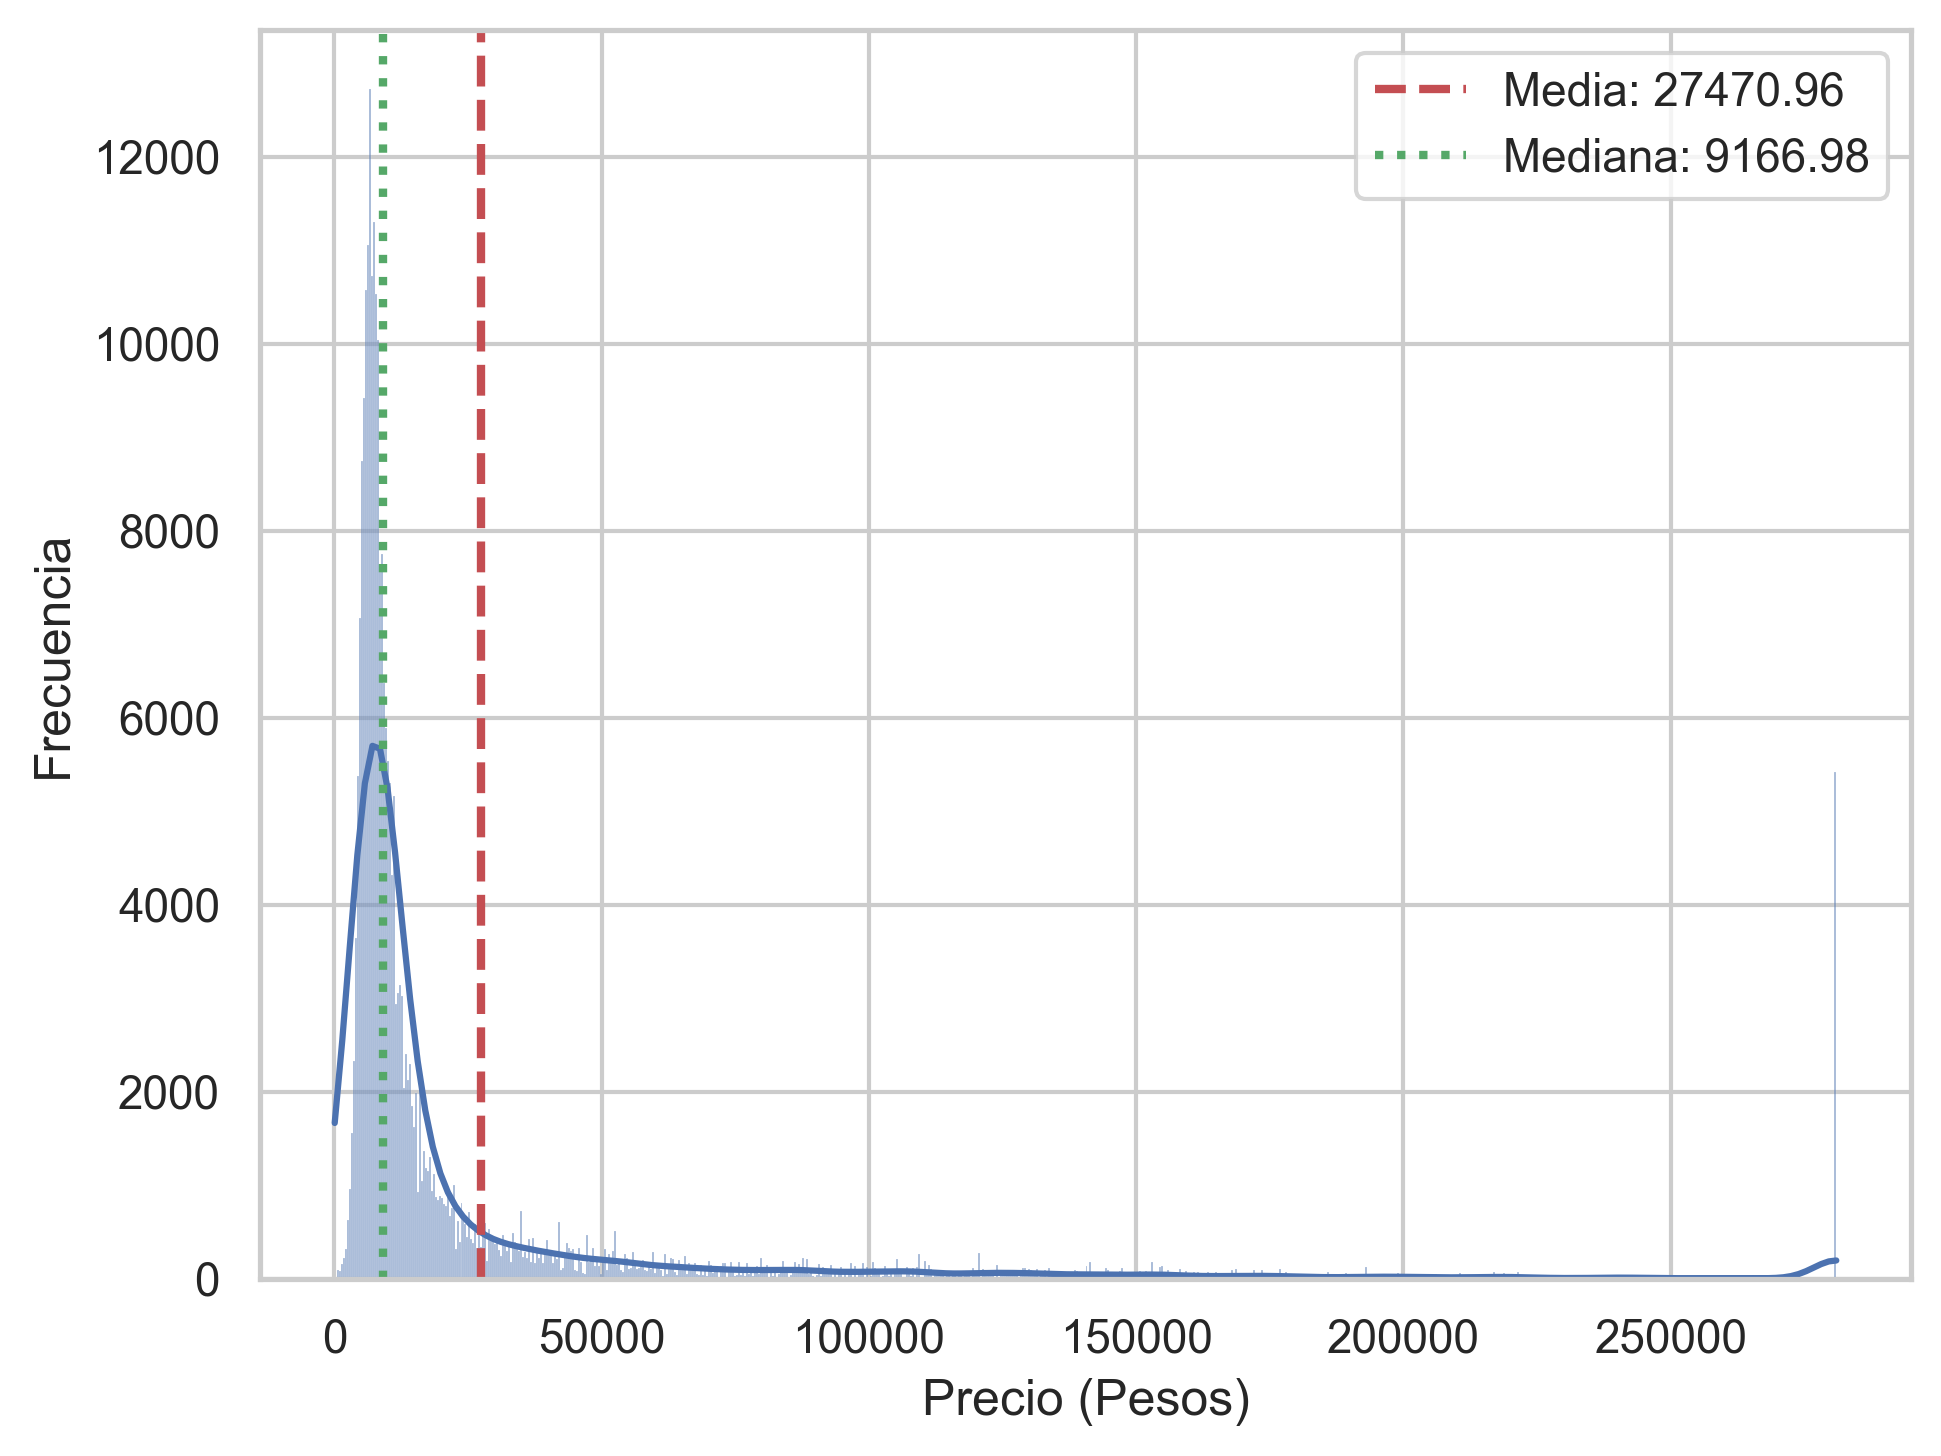
\includegraphics[width=0.95\linewidth]{plots/eda/03-distribucion-precio-clipped.png}
\end{block}

\begin{block}{Efecto Espacial y PCA por Ciudad}
\justifying
Aunque la correlación lineal entre coordenadas y precio es baja, la variabilidad espacial es evidente: las zonas cercanas al río y el corredor norte concentran los alquileres más altos. El análisis de componentes principales (PCA) coloreado por ciudad muestra gradientes continuos sin clusters netos, reflejando la heterogeneidad del mercado.

\vspace{0.15cm}
\centering
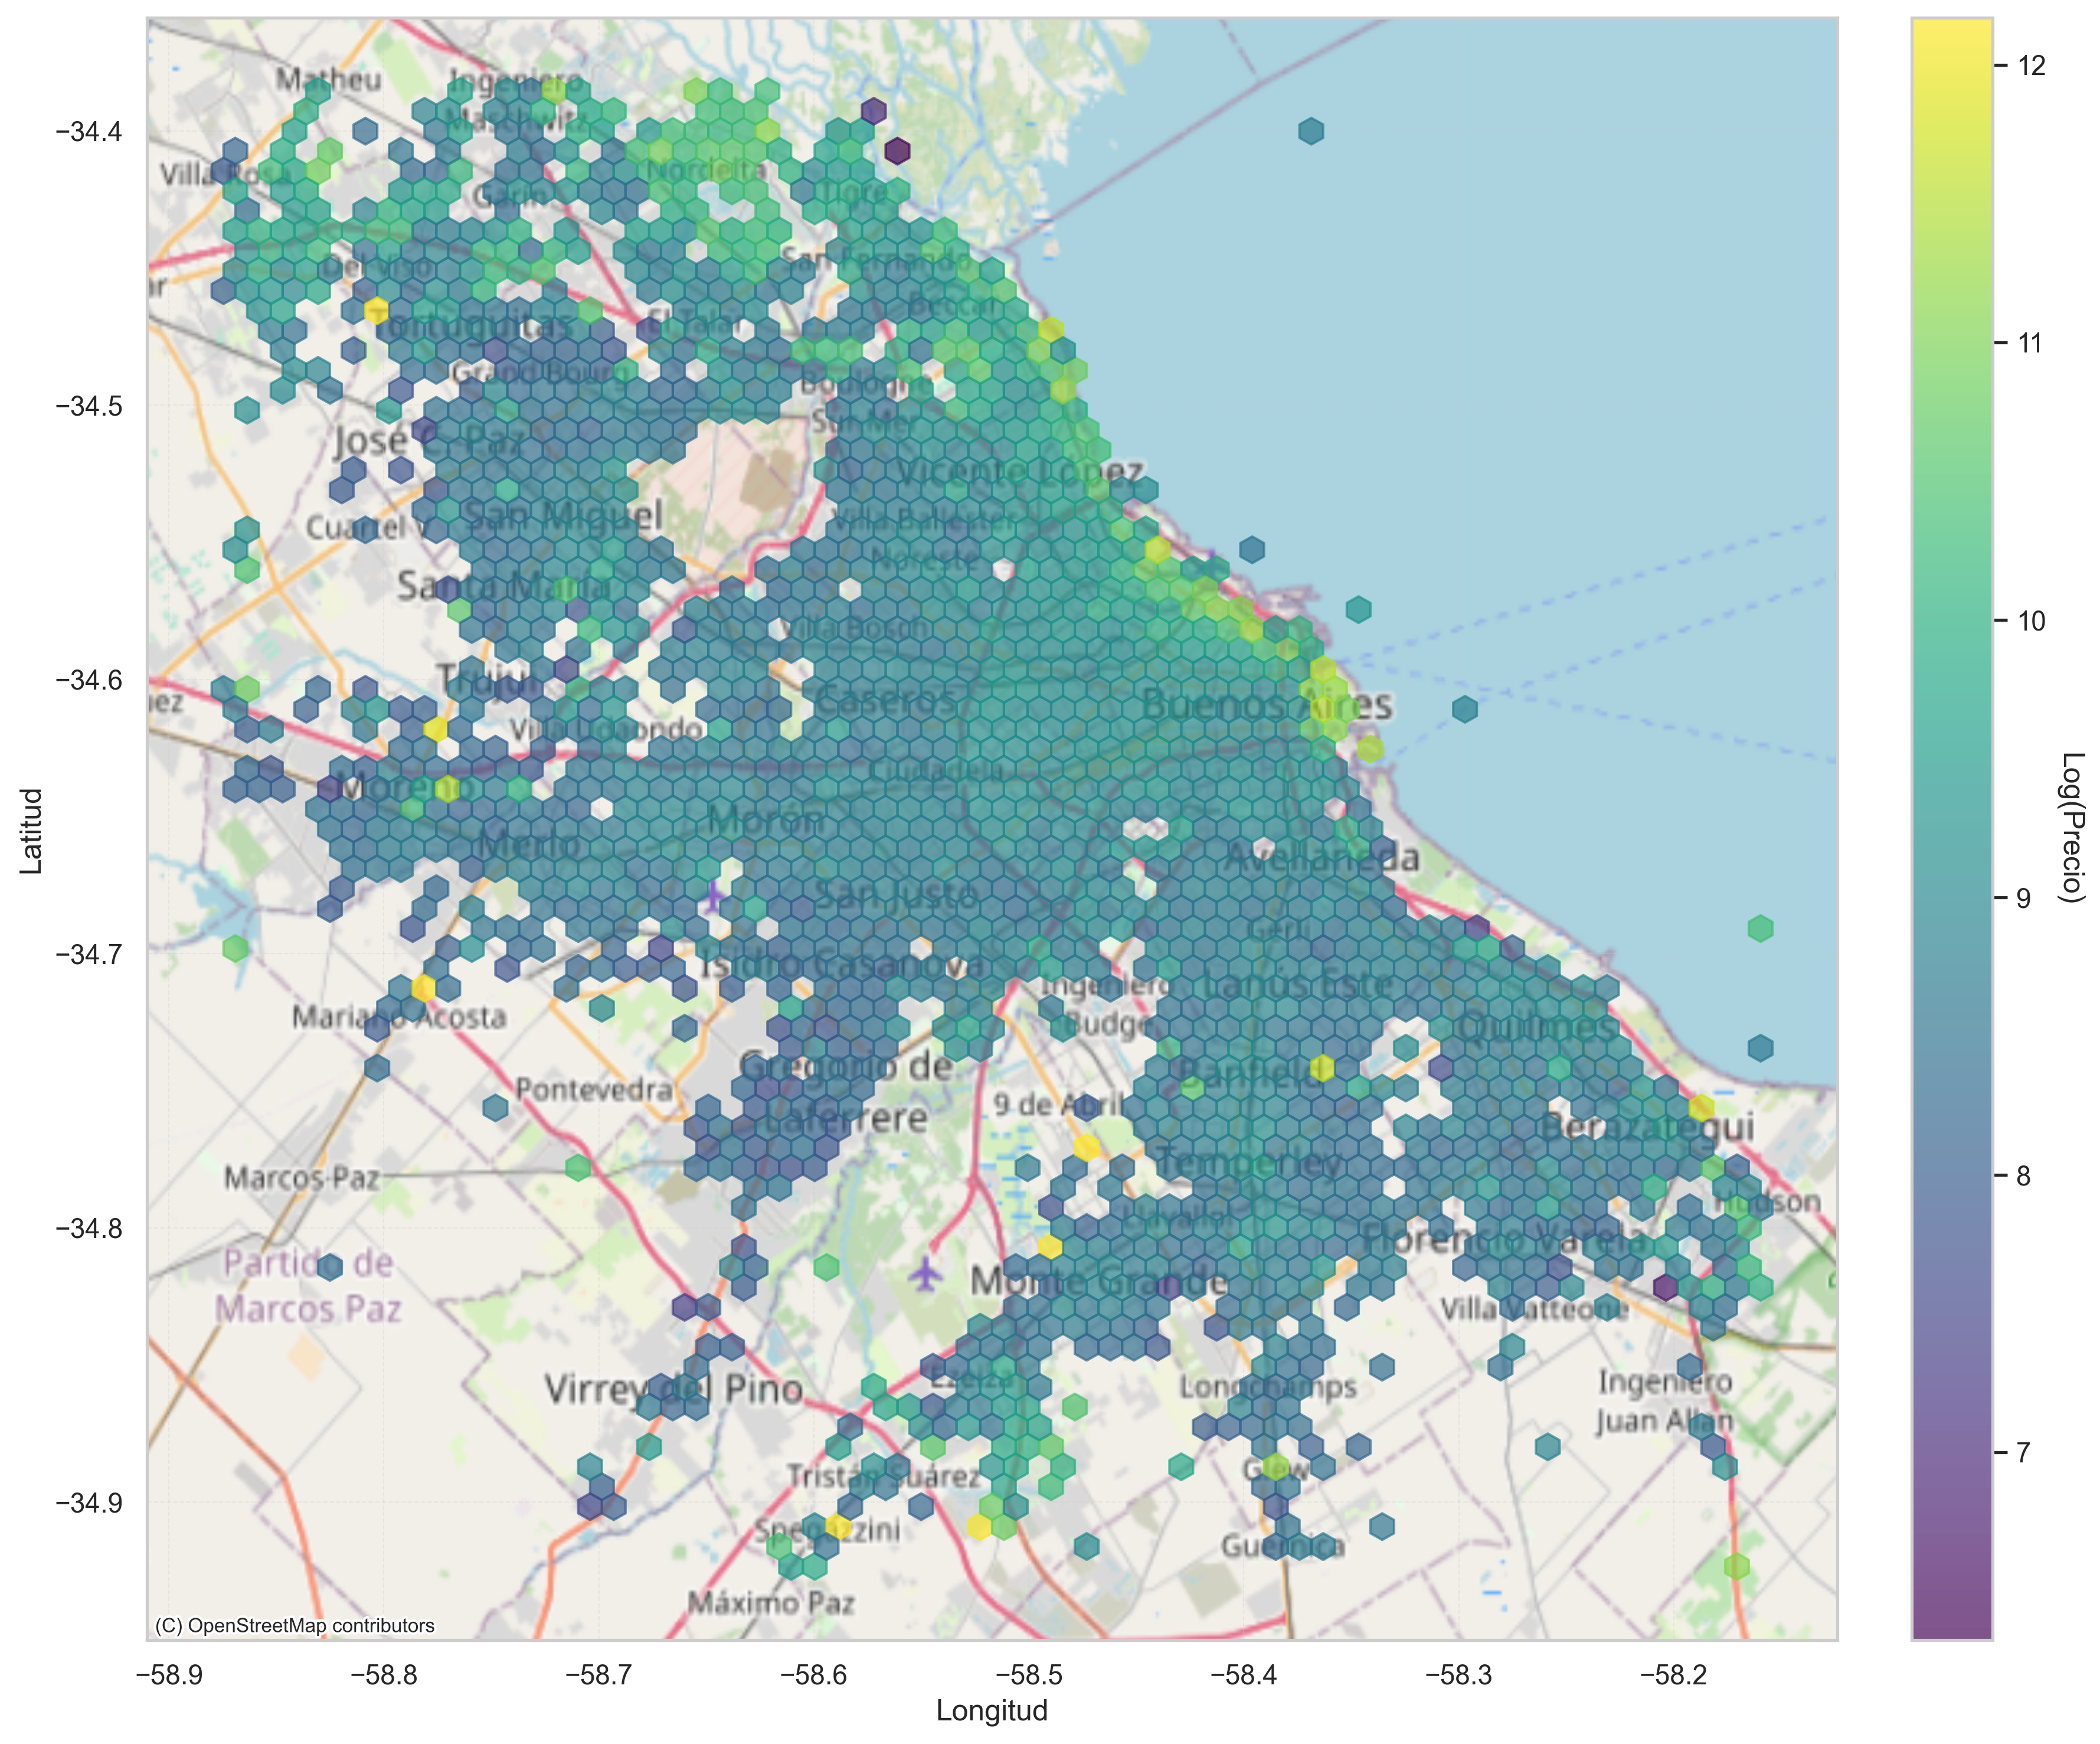
\includegraphics[width=0.95\linewidth]{plots/eda/11-geo-plot.png}

\vspace{0.25cm}
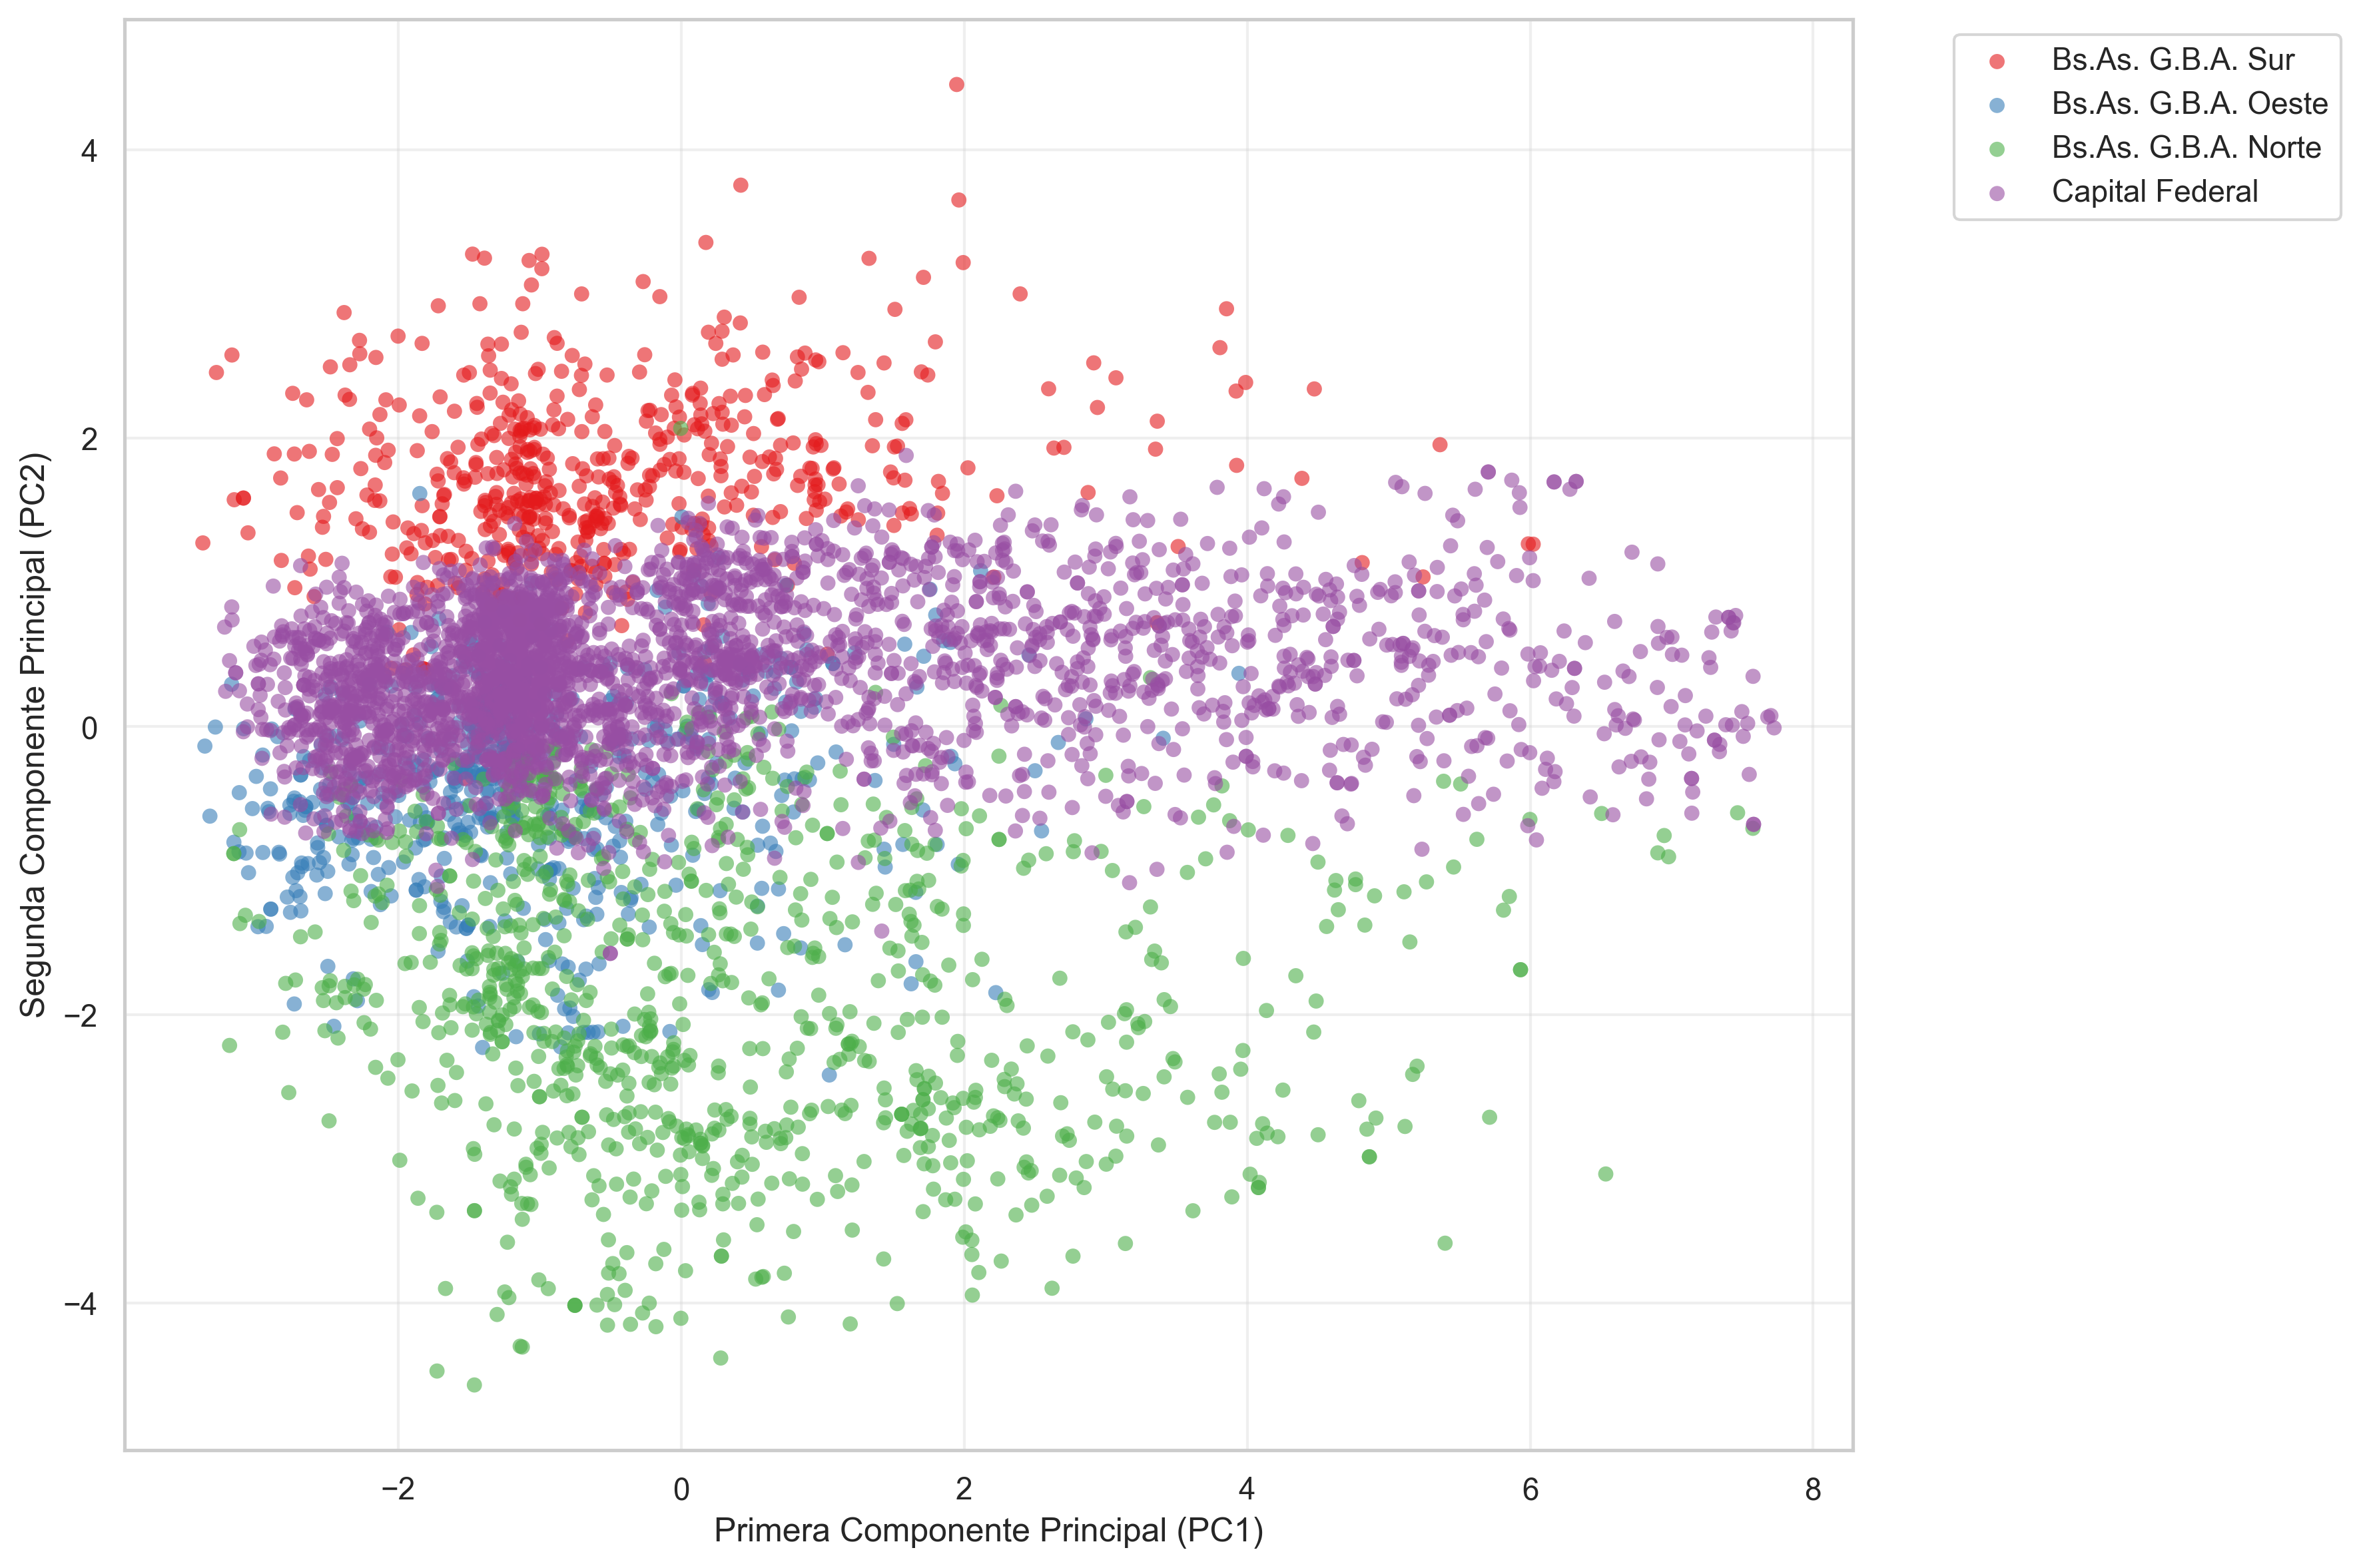
\includegraphics[width=0.95\linewidth]{plots/eda/12-pca-ciudad.png}
\end{block}

\end{column}

% =========================================================
% Column 2: Metodología y Modelo Híbrido, Comparación
% =========================================================
\begin{column}{0.33\textwidth}

\begin{block}{Metodología}
\justifying
Se construyó un \textbf{pipeline integral} de aprendizaje automático que incluye limpieza determinística, ingeniería de features (densidad de ambientes, ratio baños/dormitorios, score de amenities) e imputación adaptada a cada familia de modelos. Se evaluaron múltiples modelos: regresores baseline, \emph{gradient boosting} (XGBoost, LightGBM) y redes neuronales (MLP).

Para comprender el impacto de los outliers se trabajó con tres versiones del dataset: (i) completo, (ii) sin el 1.5\% más caro y (iii) solo el 1.5\% más caro. Este análisis guió el diseño del modelo final.
\end{block}

\begin{block}{Modelo Híbrido (Normal vs. Lujo)}
\justifying
Definimos ``lujo'' como el \textbf{percentil superior 1.5\%} del precio. El modelo híbrido desacopla dos dinámicas:
\begin{itemize}
  \item \textbf{Clasificador XGBoost} identifica si la propiedad pertenece al segmento de lujo.
  \item \textbf{Regresor normal} (XGBRegressor) predice el precio para el 98.5\% de propiedades normales.
  \item \textbf{Regresor lujo} (XGBRegressor) predice el precio para el 1.5\% de propiedades de lujo.
\end{itemize}
Esta arquitectura evita que el conjunto minoritario distorsione el aprendizaje del segmento mayoritario, sin descartar las propiedades caras.

\vspace{0.3cm}
\centering
% Diagrama del modelo híbrido
\begin{tikzpicture}[node distance=12mm, every node/.style={font=\small}]
\tikzset{
  box/.style={draw, rounded corners=8pt, align=center, inner sep=4pt, font=\small, minimum width=1.9cm},
  arrow/.style={-Latex, line width=0.8pt}
}

% Nodes
\node[box] (feat) {\textbf{Features}\newline Superficie, amenities, ubicación, tiempo};
\node[box, below=of feat] (clf) {\textbf{Clasificador}\newline XGBoost};
\node[box, below left=12mm and 7mm of clf] (regN) {\textbf{Regresor Normal}\newline XGBRegressor};
\node[box, below right=12mm and 7mm of clf] (regL) {\textbf{Regresor Lujo}\newline XGBRegressor};

% Arrows
\draw[arrow] (feat) -- (clf);
\draw[arrow] (clf) -- node[left, font=\scriptsize] {No lujo} (regN);
\draw[arrow] (clf) -- node[right, font=\scriptsize] {Lujo} (regL);
\end{tikzpicture}
\end{block}

\begin{block}{Comparación de Modelos}
\justifying
La figura resume las métricas obtenidas en test. El modelo híbrido alcanza el \textbf{mejor MAE} y \textbf{MedAE}, reduciendo el error típico en el mercado masivo. Un XGBoost único optimizado logra un RMSE ligeramente menor, reflejando un mejor ajuste a los errores extremos. Este contraste confirma el trade--off entre precisión promedio y penalización de extremos.
\vspace{0.25cm}
\centering
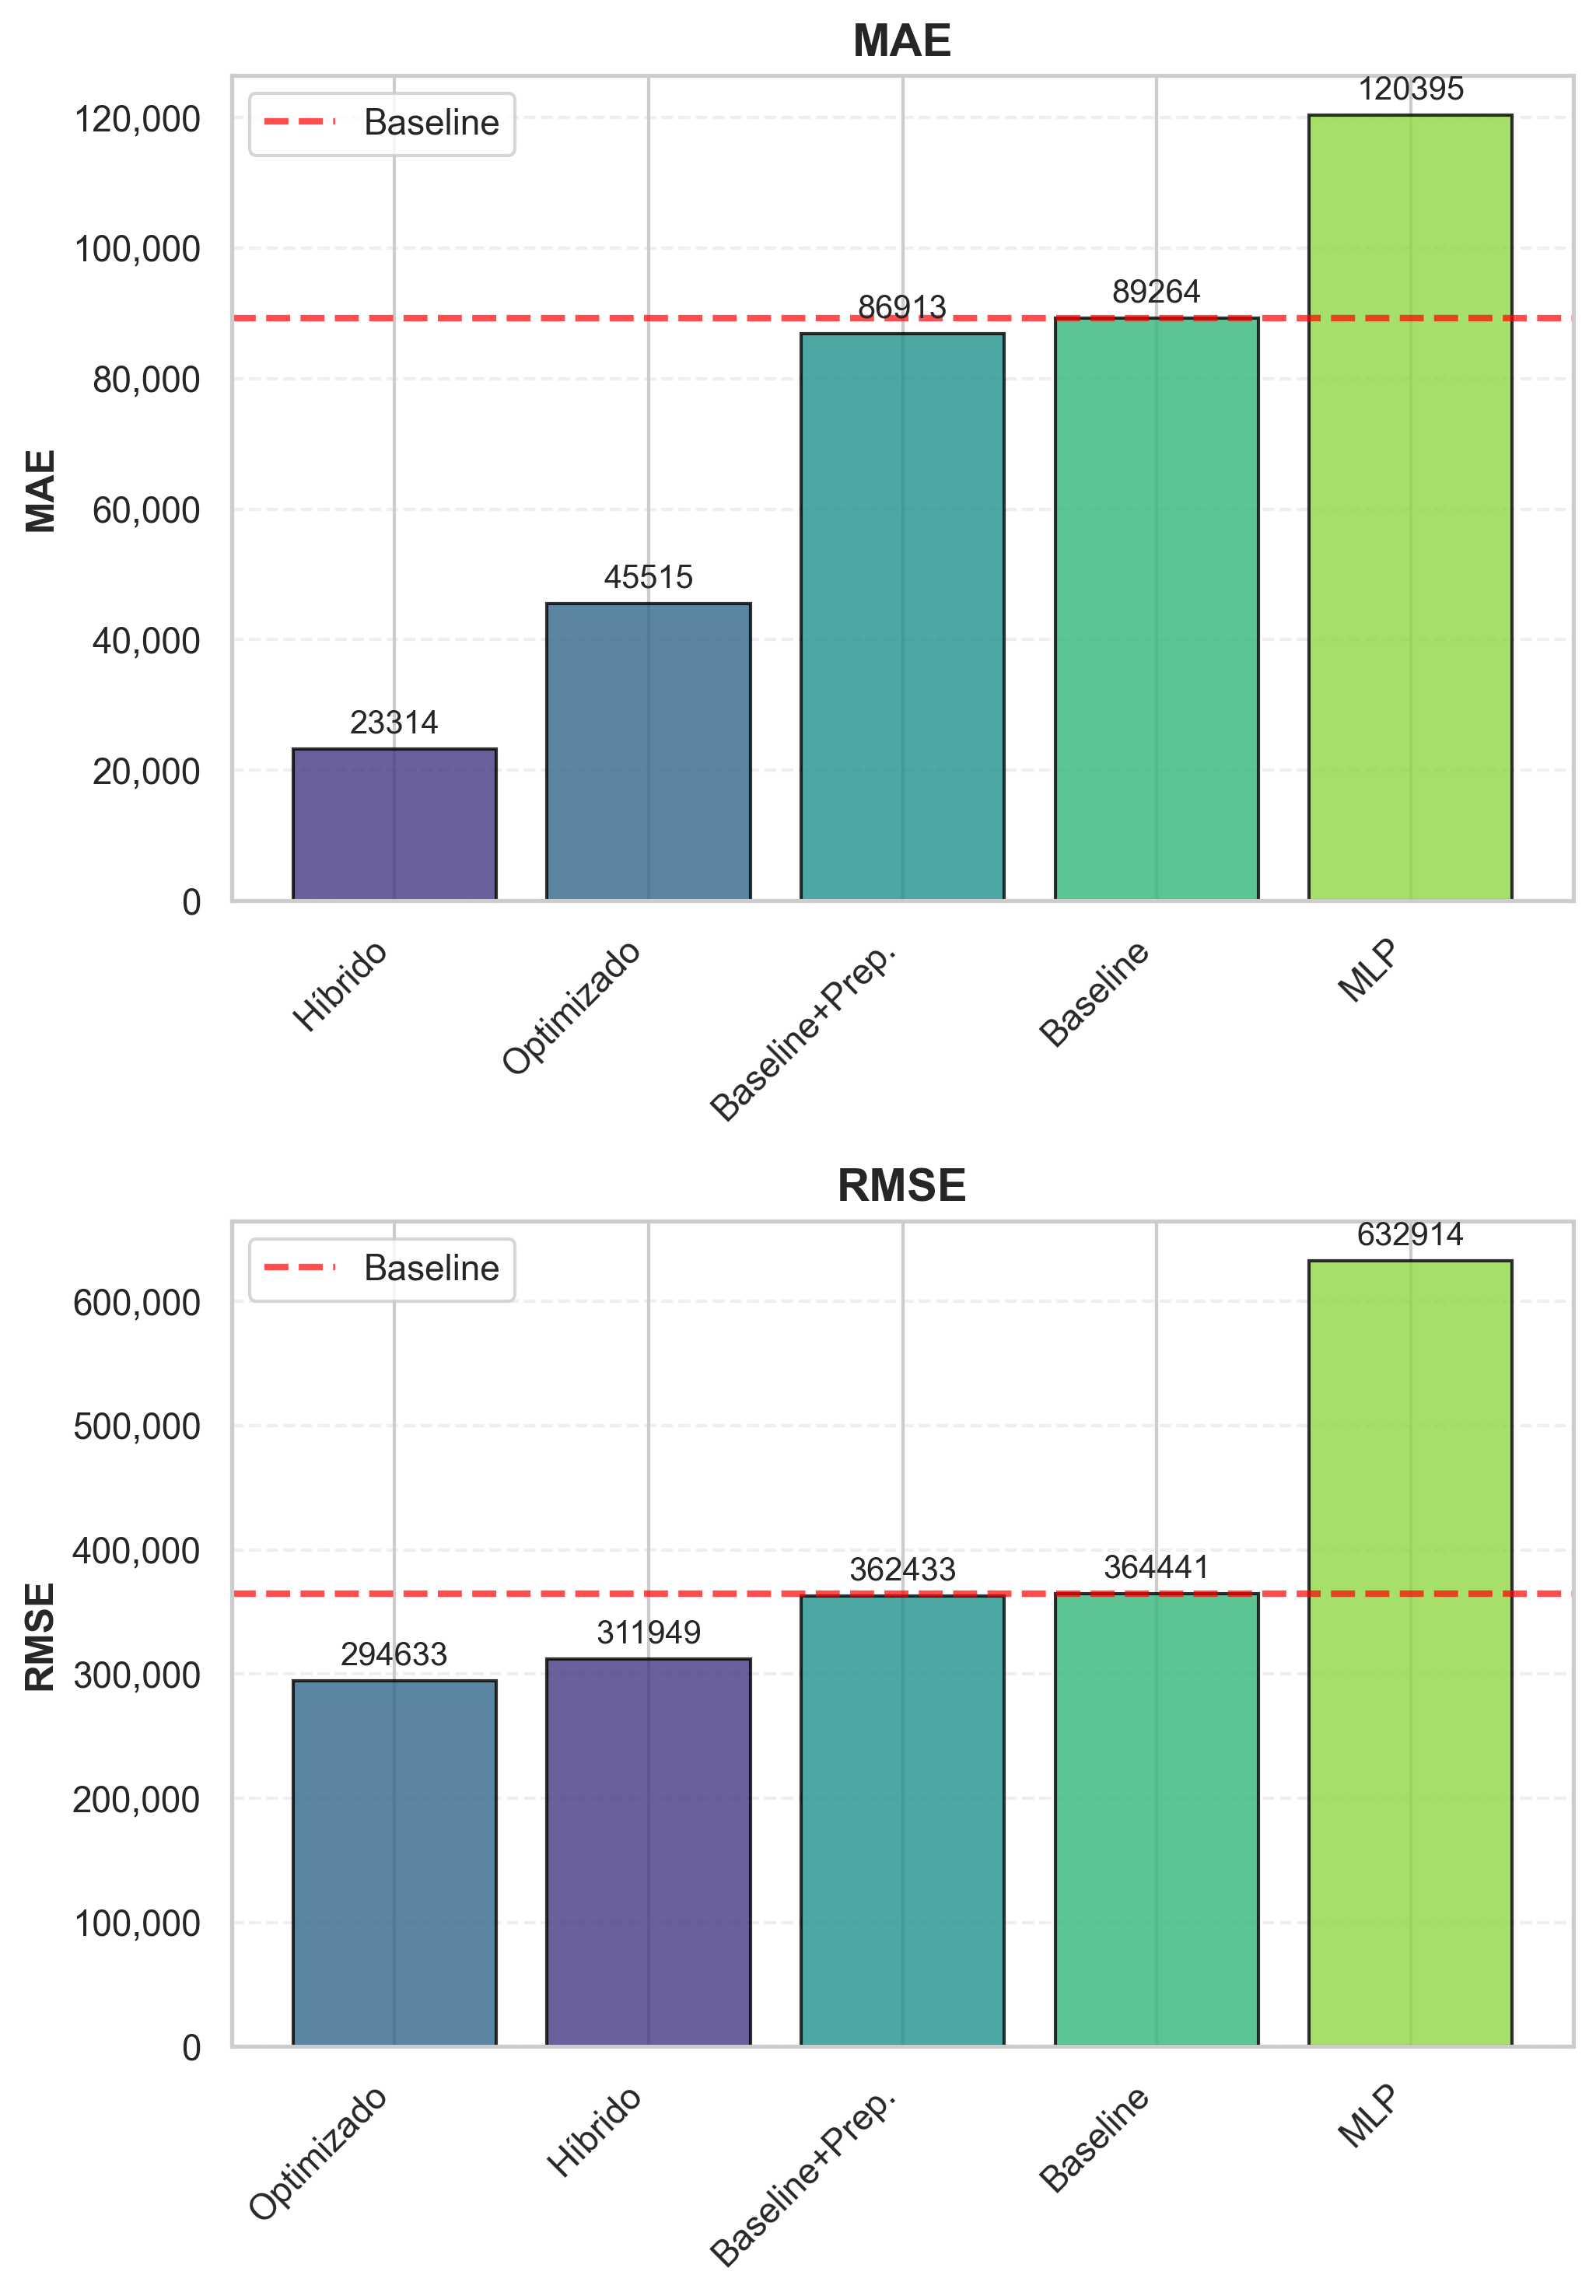
\includegraphics[width=0.95\linewidth]{plots/01-comparacion-final.png}
\end{block}

\end{column}

% =========================================================
% Column 3: SHAP, Impacto amenities, Conclusión
% =========================================================
\begin{column}{0.33\textwidth}

\begin{block}{Importancia de Variables (SHAP)}
\justifying
Para interpretar el modelo se emplearon valores SHAP, descomponiendo cada predicción en contribuciones de las features. La \textbf{superficie construida} y las variables de habitabilidad son los principales determinantes del precio, seguidos por la ubicación geográfica. Esta explicación confirma que el modelo captura interacciones no lineales coherentes con la estructura del mercado.
\vspace{0.25cm}
\centering
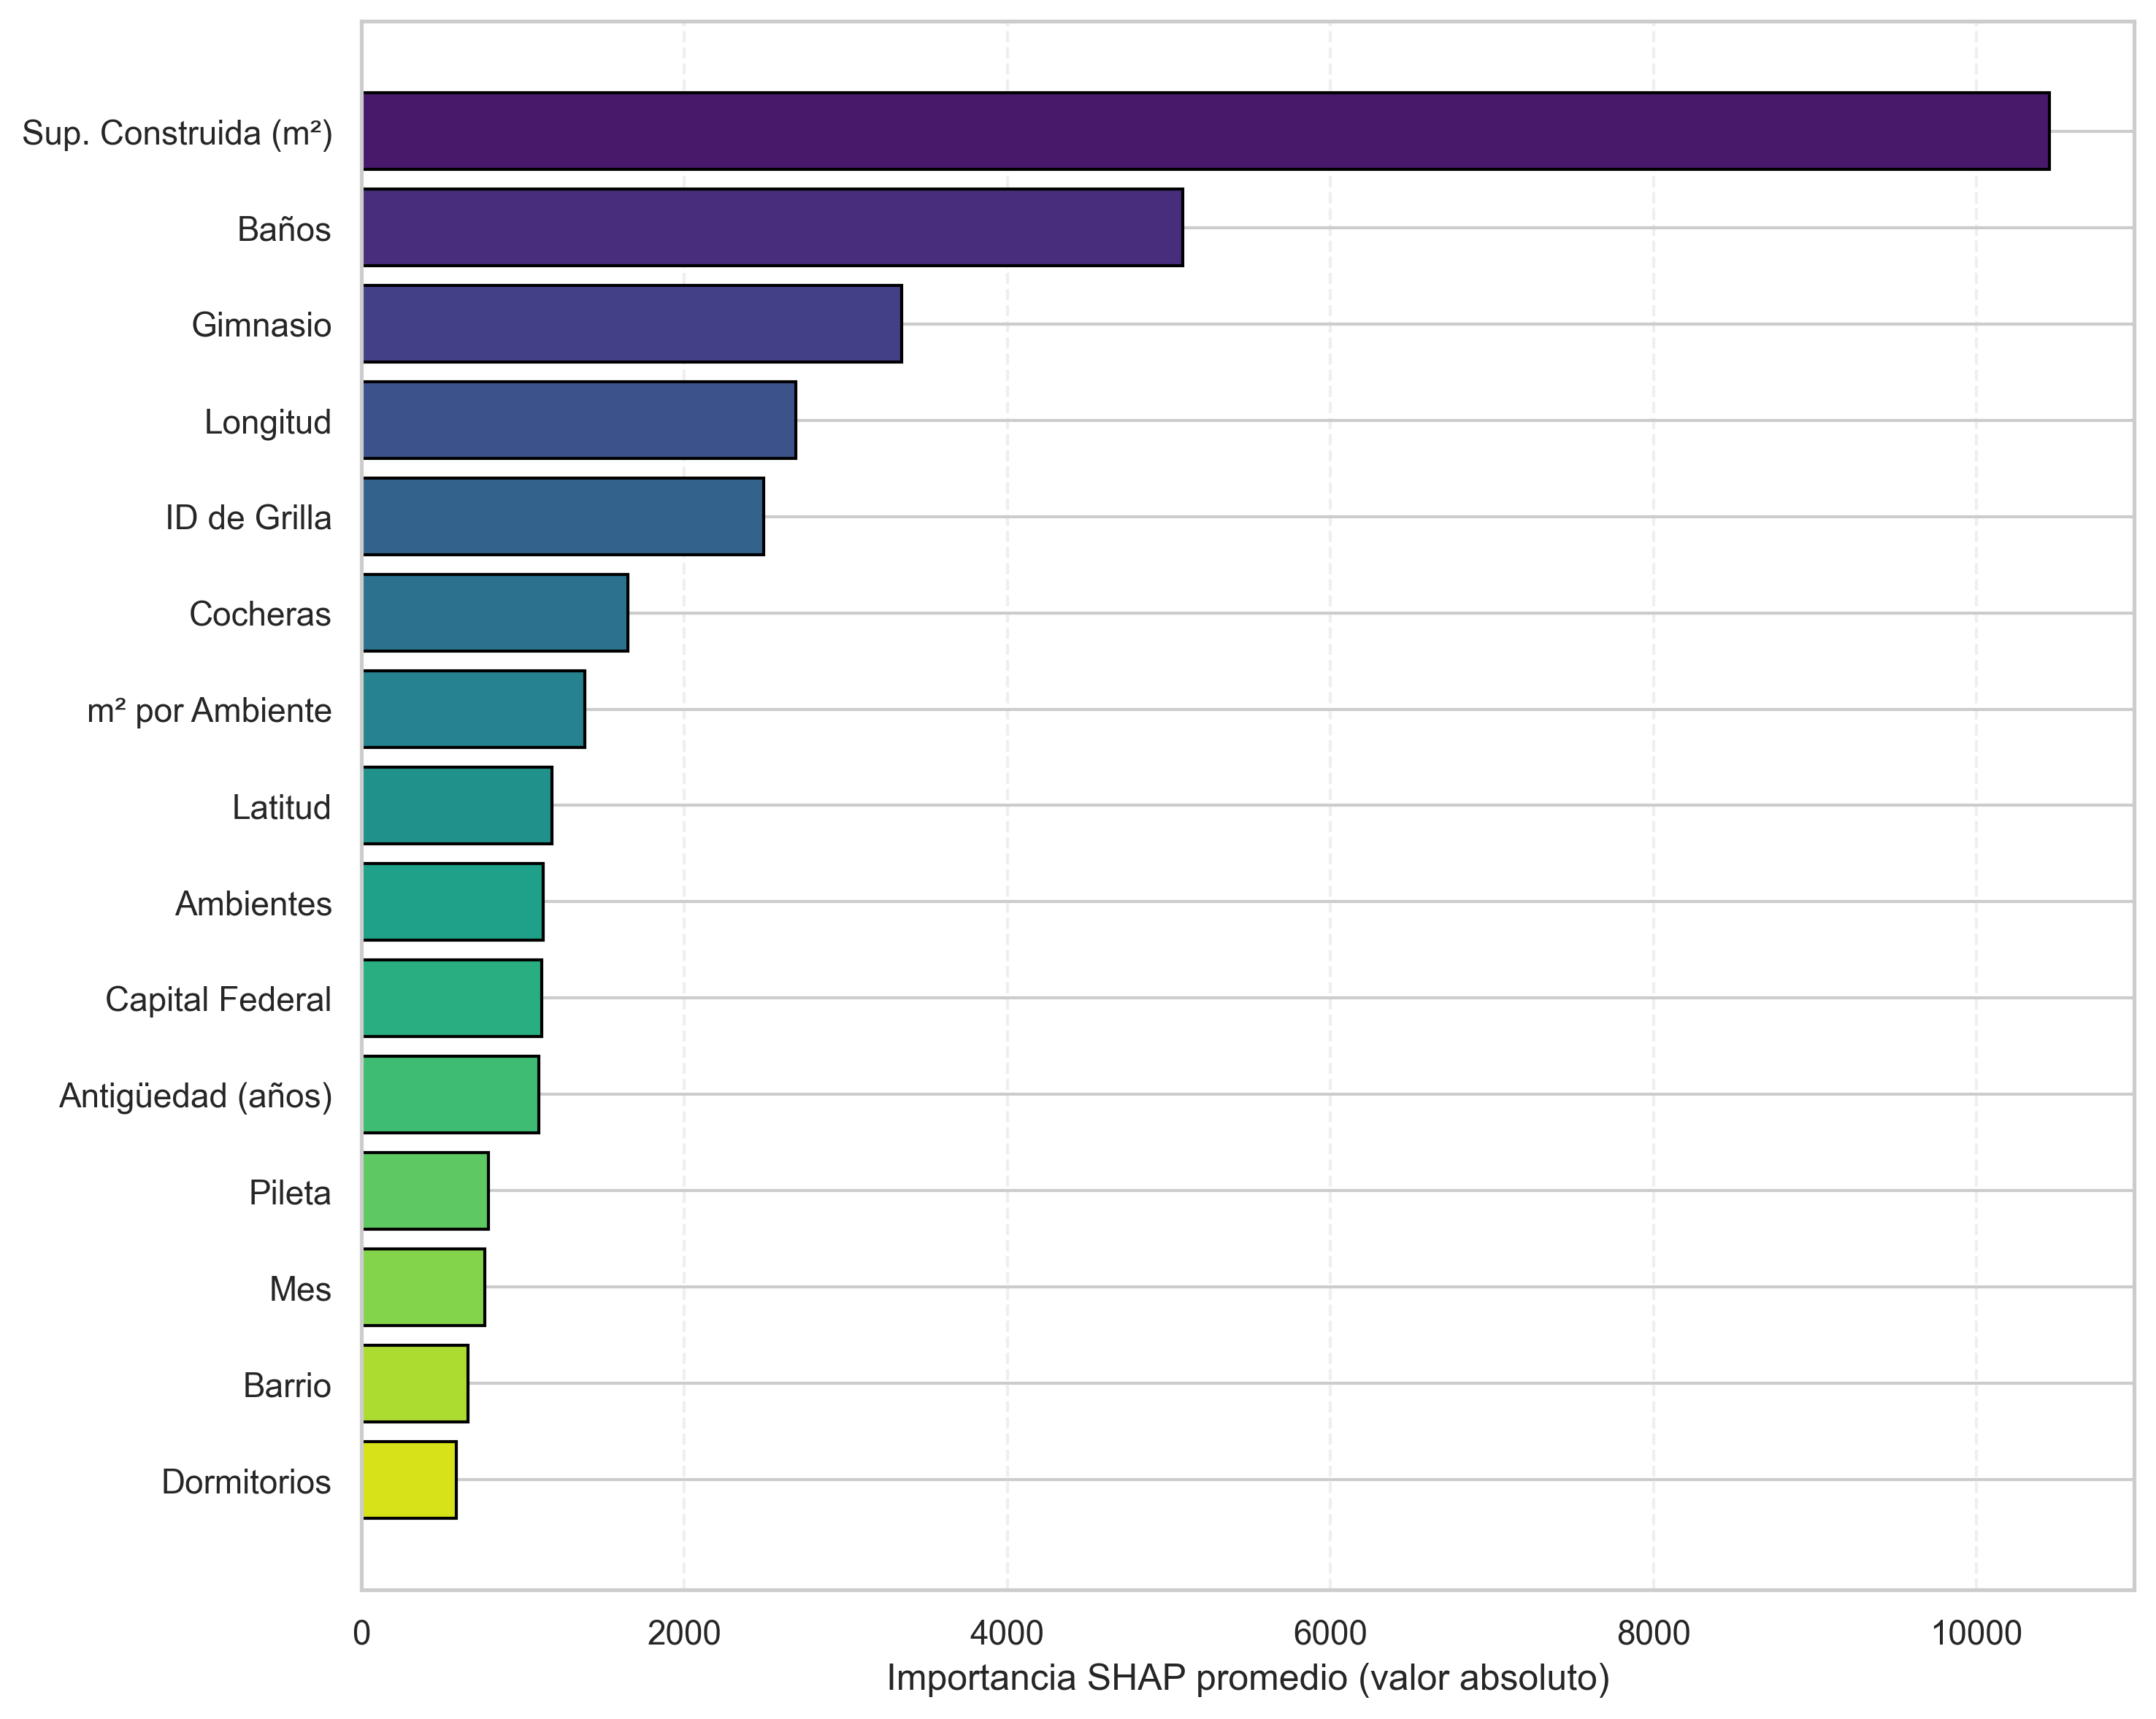
\includegraphics[width=0.95\linewidth]{plots/analisis-explicativo/01-feature-importance.png}
\end{block}

\begin{block}{Impacto de Amenities por Zona}
\justifying
El análisis SHAP por zona revela que las \textbf{amenities premium} (gimnasio, pileta, seguridad) no tienen el mismo valor en todo el AMBA. En Capital Federal y zona norte su efecto sobre el precio es significativamente mayor que en el conurbano sur u oeste, reflejando diferencias socioeconómicas y de oferta inmobiliaria.
\vspace{0.25cm}
\centering
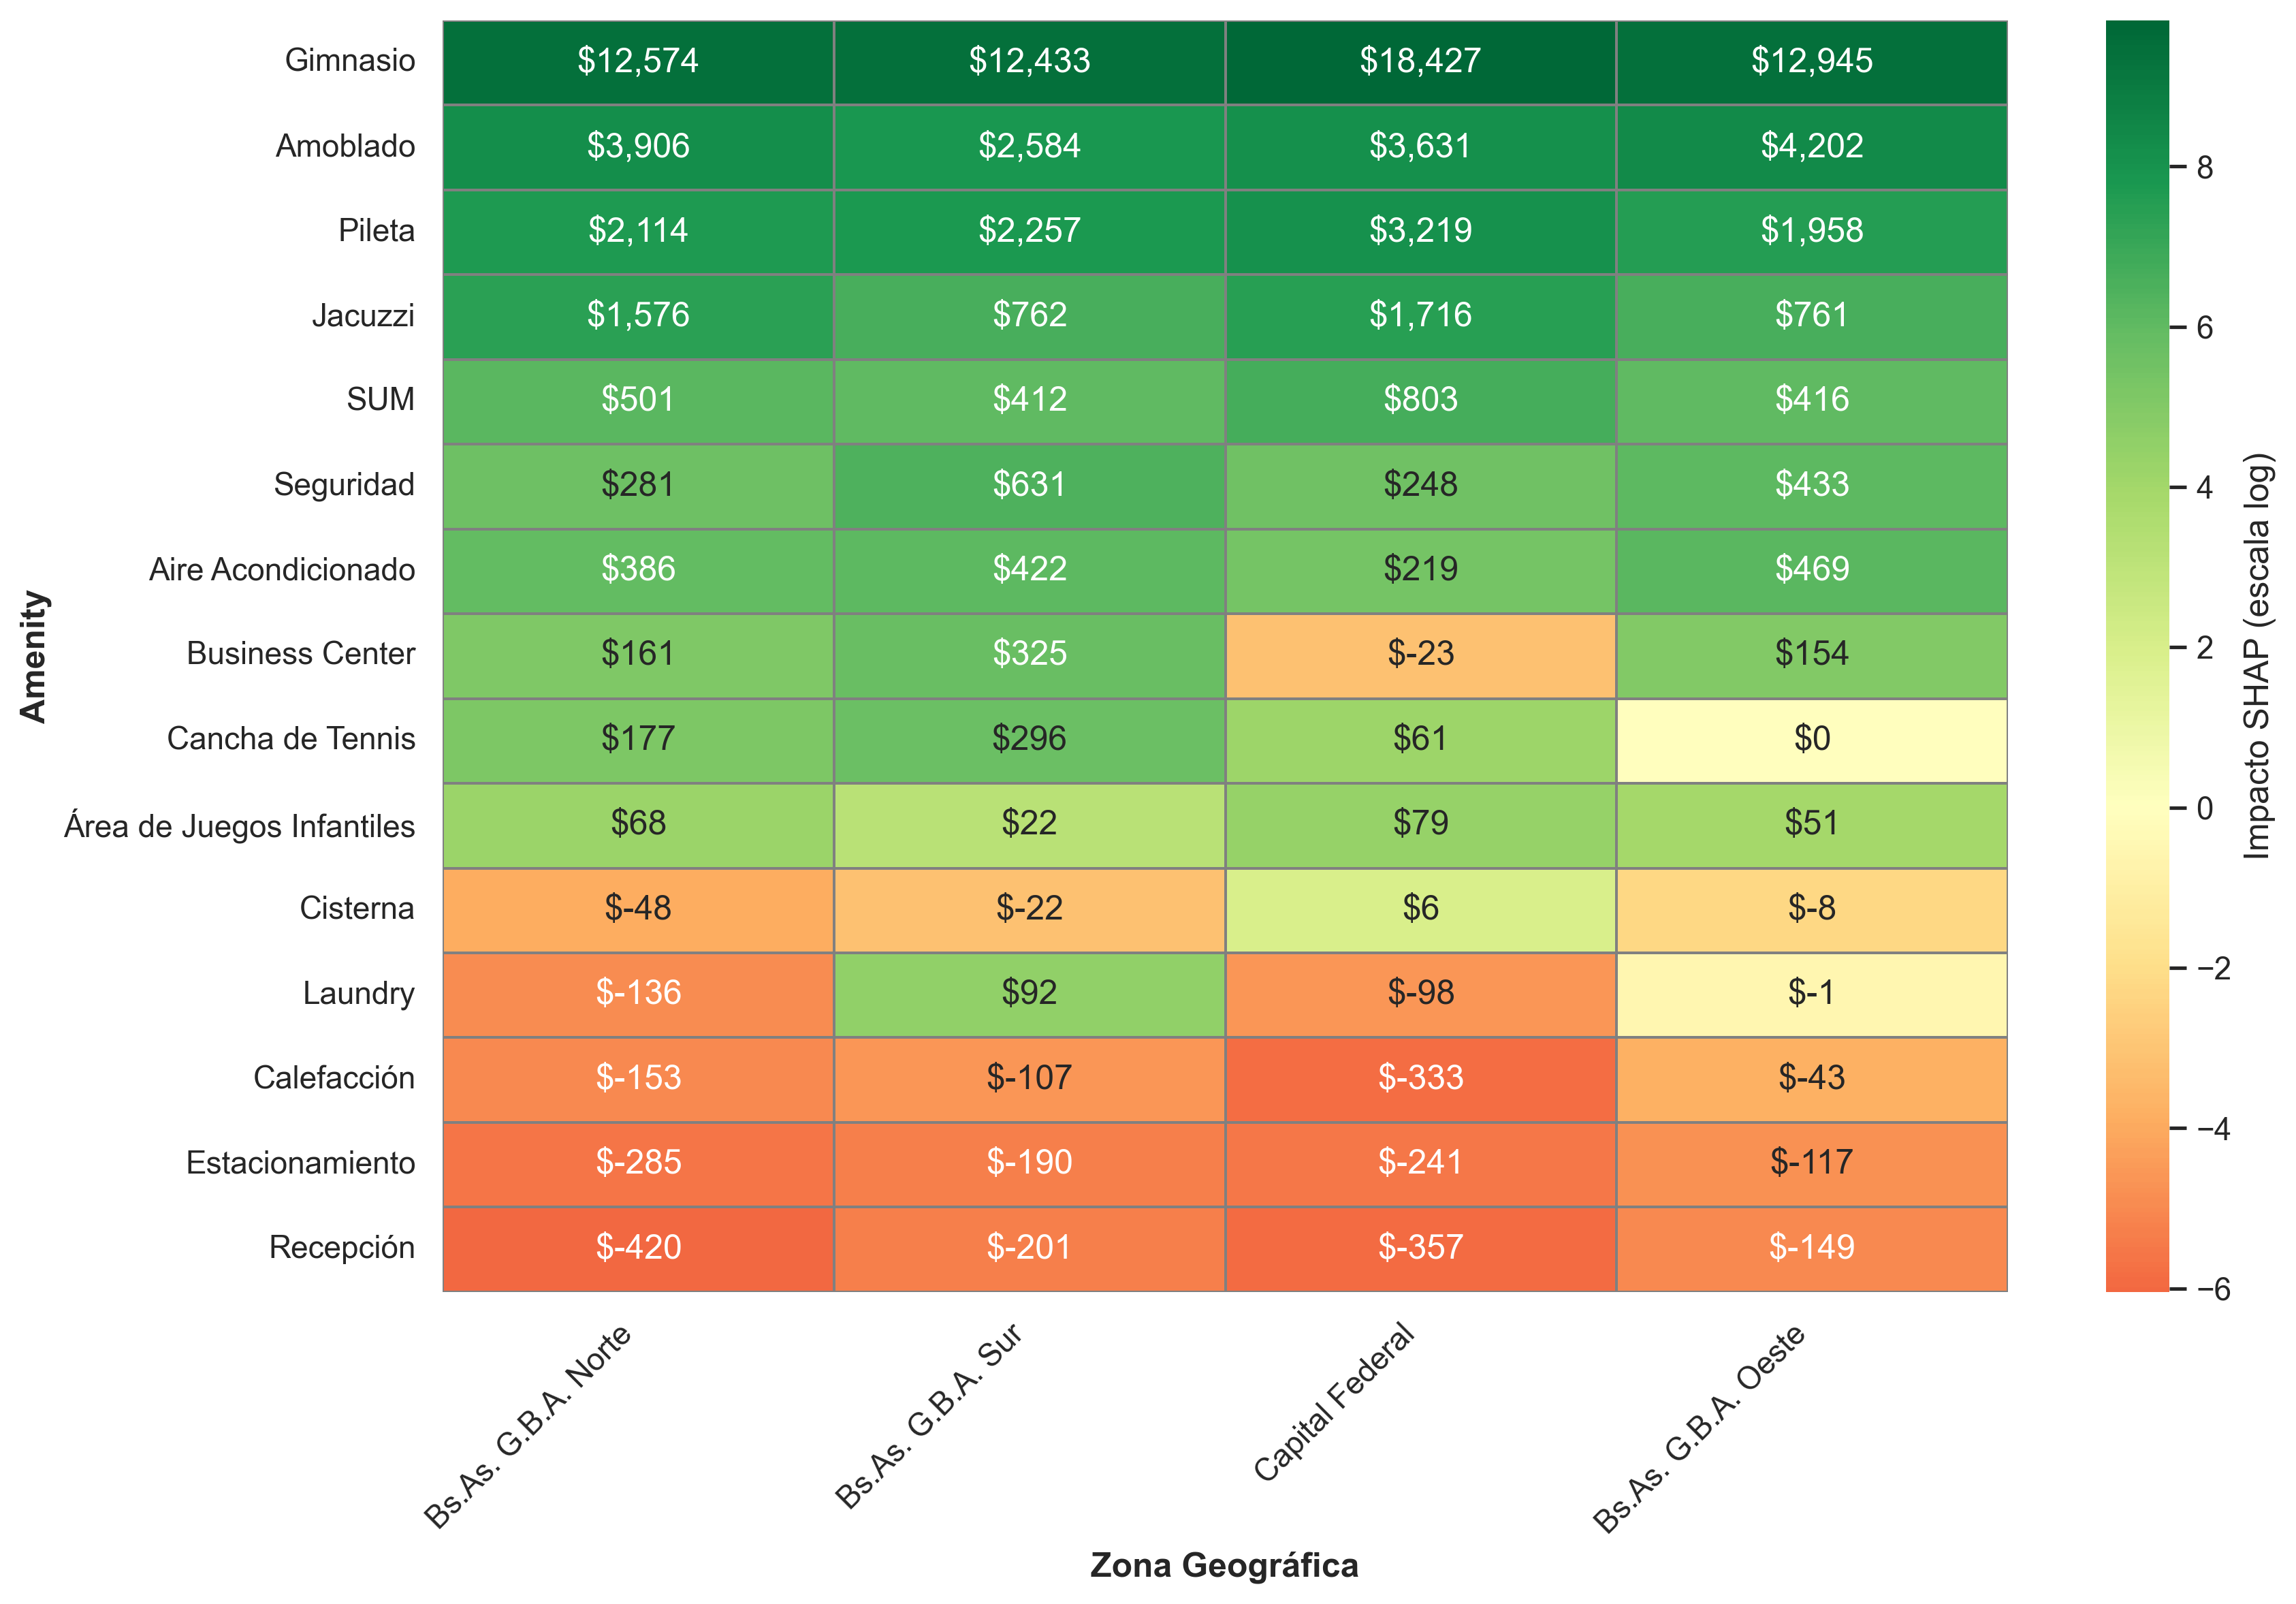
\includegraphics[width=0.95\linewidth]{plots/analisis-explicativo/03-amenities-impact-per-state.png}
\end{block}

\begin{block}{Conclusiones y Futuro}
\justifying
\textbf{Conclusión:} segmentar el mercado y entrenar regresores especializados mejora drásticamente la precisión en el segmento masivo sin desechar las propiedades de lujo. El modelo híbrido es la mejor elección cuando se prioriza el error típico (MAE/MedAE); un XGBoost único optimizado es preferible si el objetivo es reducir el RMSE.

\textbf{Líneas futuras:} (1) Diseñar un tercer experto para ultra-lujo y detectar anomalías; (2) incorporar datos externos socioeconómicos y de accesibilidad; (3) explorar modelos \emph{mixture-of-experts} entrenados de forma conjunta y calibrar mejor el clasificador.

\vspace{0.25cm}
\textbf{Repositorio:} \url{https://github.com/gonzabaleta/alquileres}
\end{block}

\end{column}

\end{columns}
\end{frame}
\end{document}